\section{Performance}

After the calibration constants are determined, the timing, position, and deposited energy of each hit are reconstructed, and clusters are formed grouping hits according to their position and timing~\cite{recon-nim}.

Data taken during the first CLAS12 experiments on hydrogen and deuterium targets, and with various beam energies (7.5 and 10.6 GeV), were analyzed to verify the performance of the CND. 

The timing performance for the three layers of the CND is illustrated in Fig.~\ref{fig_performance_deltat_layers}, showing the vertex time difference $v_t$ for selected negative tracks, assumed to be all pions, integrated over all sectors defined as
\begin{equation}\label{eq_vtp_definition}
v_t=t_{\rm{CND}}-(t_{\rm{S}}-vz_{corr})-\frac{P_L}{c \cdot \beta} ,
\end{equation}
where $t_{\rm{CND}}$ is the mean time reconstructed from the L and R paddles, $t_{\rm{S}}$ is the event start time determined by the RF bucket matched with the FTOF vertex time, $vz_{corr}$ accounts for the actual $z$ position of the interaction vertex, $P_L$ is the path length from the event vertex to the CND, and
\begin{equation}\label{eq_beta_definition}
  \beta=\frac{p}{\sqrt{p^2+m^2}},
\end{equation}
with $p$ the momentum measured by the CVT, and $m$ the pion mass. 
The distribution of $v_t$ is centered at 0. From the width of the $v_t$ distribution the timing resolution of each CND paddle convoluted with the CVT resolution can be determined as:
\begin{equation}\label{eq_resolution}
\sigma_t=\sqrt{\sigma_{v_t}^2-\sigma_{t_{S}}^2}=0 , 185~\rm{ps}, 
\end{equation}
assuming the resolution of the start time $\sigma_{t_{S}}$=20~ps~\cite{ftof-nim}.
%This is compatible with the detector specifications (150 ps) and the result of the measurements in cosmic rays during the detector assembly phase \cite{Niccolai:2018qzm} (148 ps).
The timing resolution for the 144 individual CND counters is shown in Fig.~\ref{fig_performance_vt_sigma_allpaddles}. Its average (indicated by the horizontal line) is around 185~ps, which is more than the average148~ps  intrinsic timing resolution measured with cosmic rays~\cite{Niccolai:2018qzm}. This discrepancy is due to multiple factors, such as the current, not fully optimized, quality of the calibrations and reconstruction, as well as the uncertainty of the path length and on the other non-CND contributions to Eq.~\ref{eq_vtp_definition}.
\begin{figure}[htb]  
\begin{center}
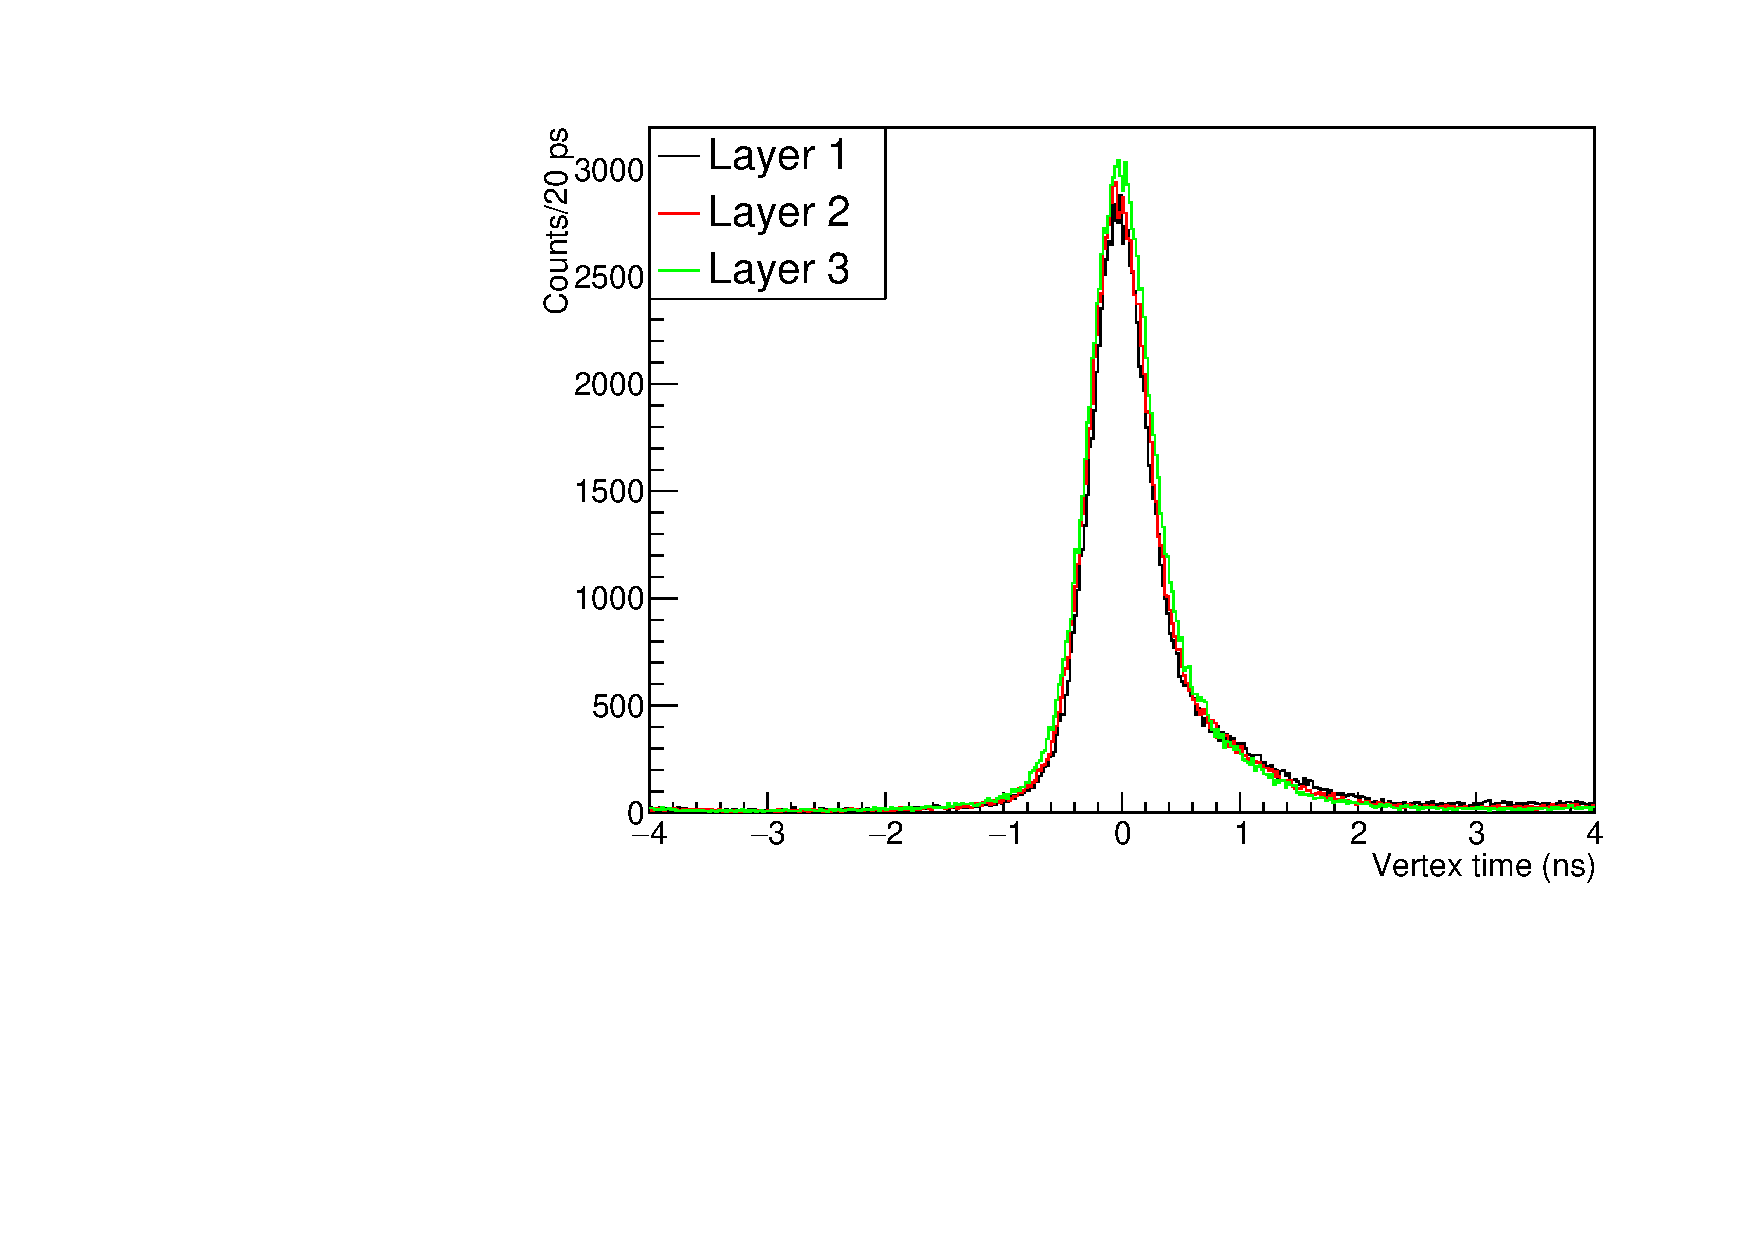
\includegraphics[width=0.45\textwidth]{Figure/canVTPlot.pdf}
\caption {Difference between the vertex time computed combining CND and CVT information with the start time computed by the FTOF for negative tracks in all the three layers of the CND integrated over all paddles.}
\label{fig_performance_deltat_layers}
\end{center}
\end{figure}

\begin{figure}[htb]  
\begin{center}
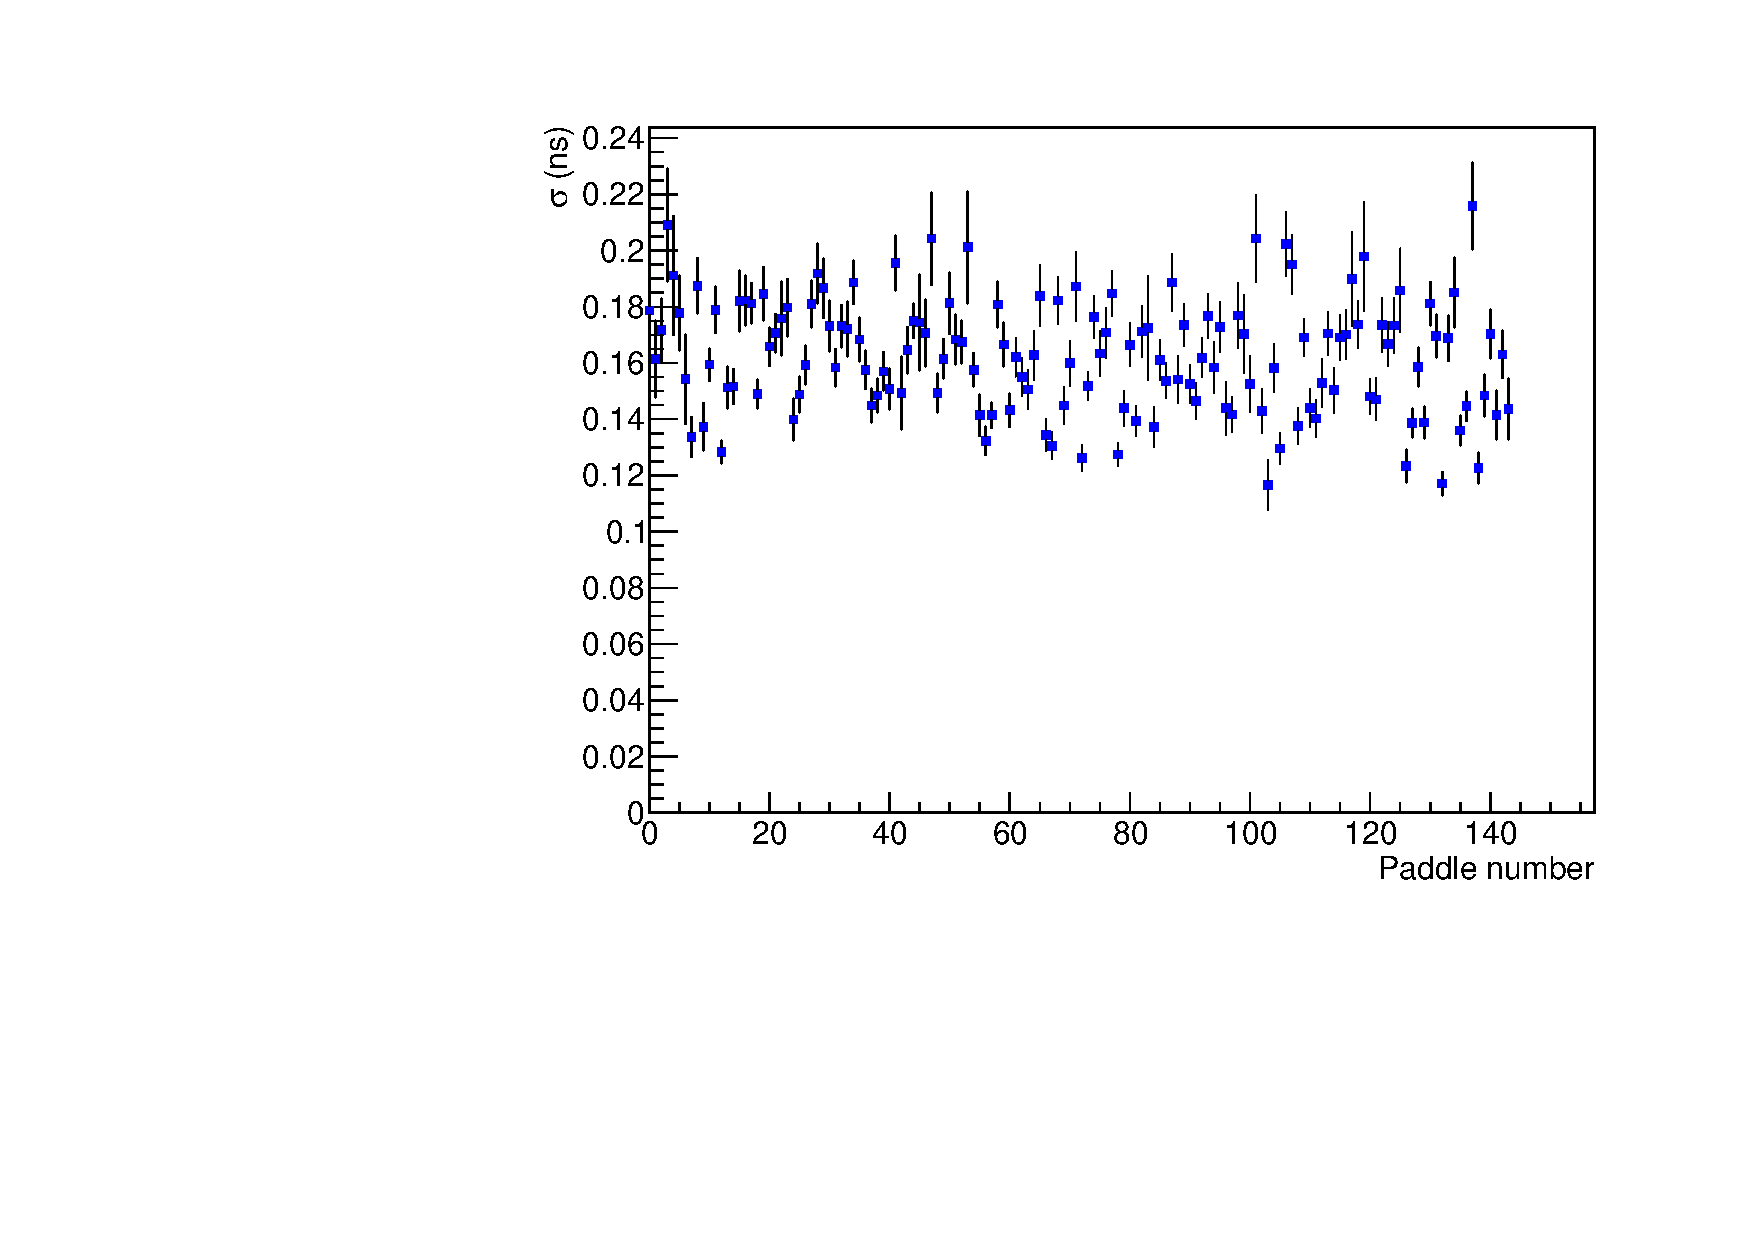
\includegraphics[width=0.45\textwidth]{Figure/VTsigma.pdf}
\caption {Timing resolution for each CND counter convoluted with the CVT resolution.}
\label{fig_performance_vt_sigma_allpaddles}
\end{center}
\end{figure}

The position reconstruction performance of the CND is shown in Fig.~\ref{fig_performance_deltaz}, which displays the difference between the $z$ coordinate (along the beamline) computed by the CND and by the CVT for negative tracks in all
three layers of the CND integrated over all paddles. Its Gaussian width is $\sim$3~cm, corresponding roughly to $4^\circ$ in polar-angle resolution. This corresponds to the convolution of the angular resolutions of the CND and CVT. 

\begin{figure}[htb]  
\begin{center}
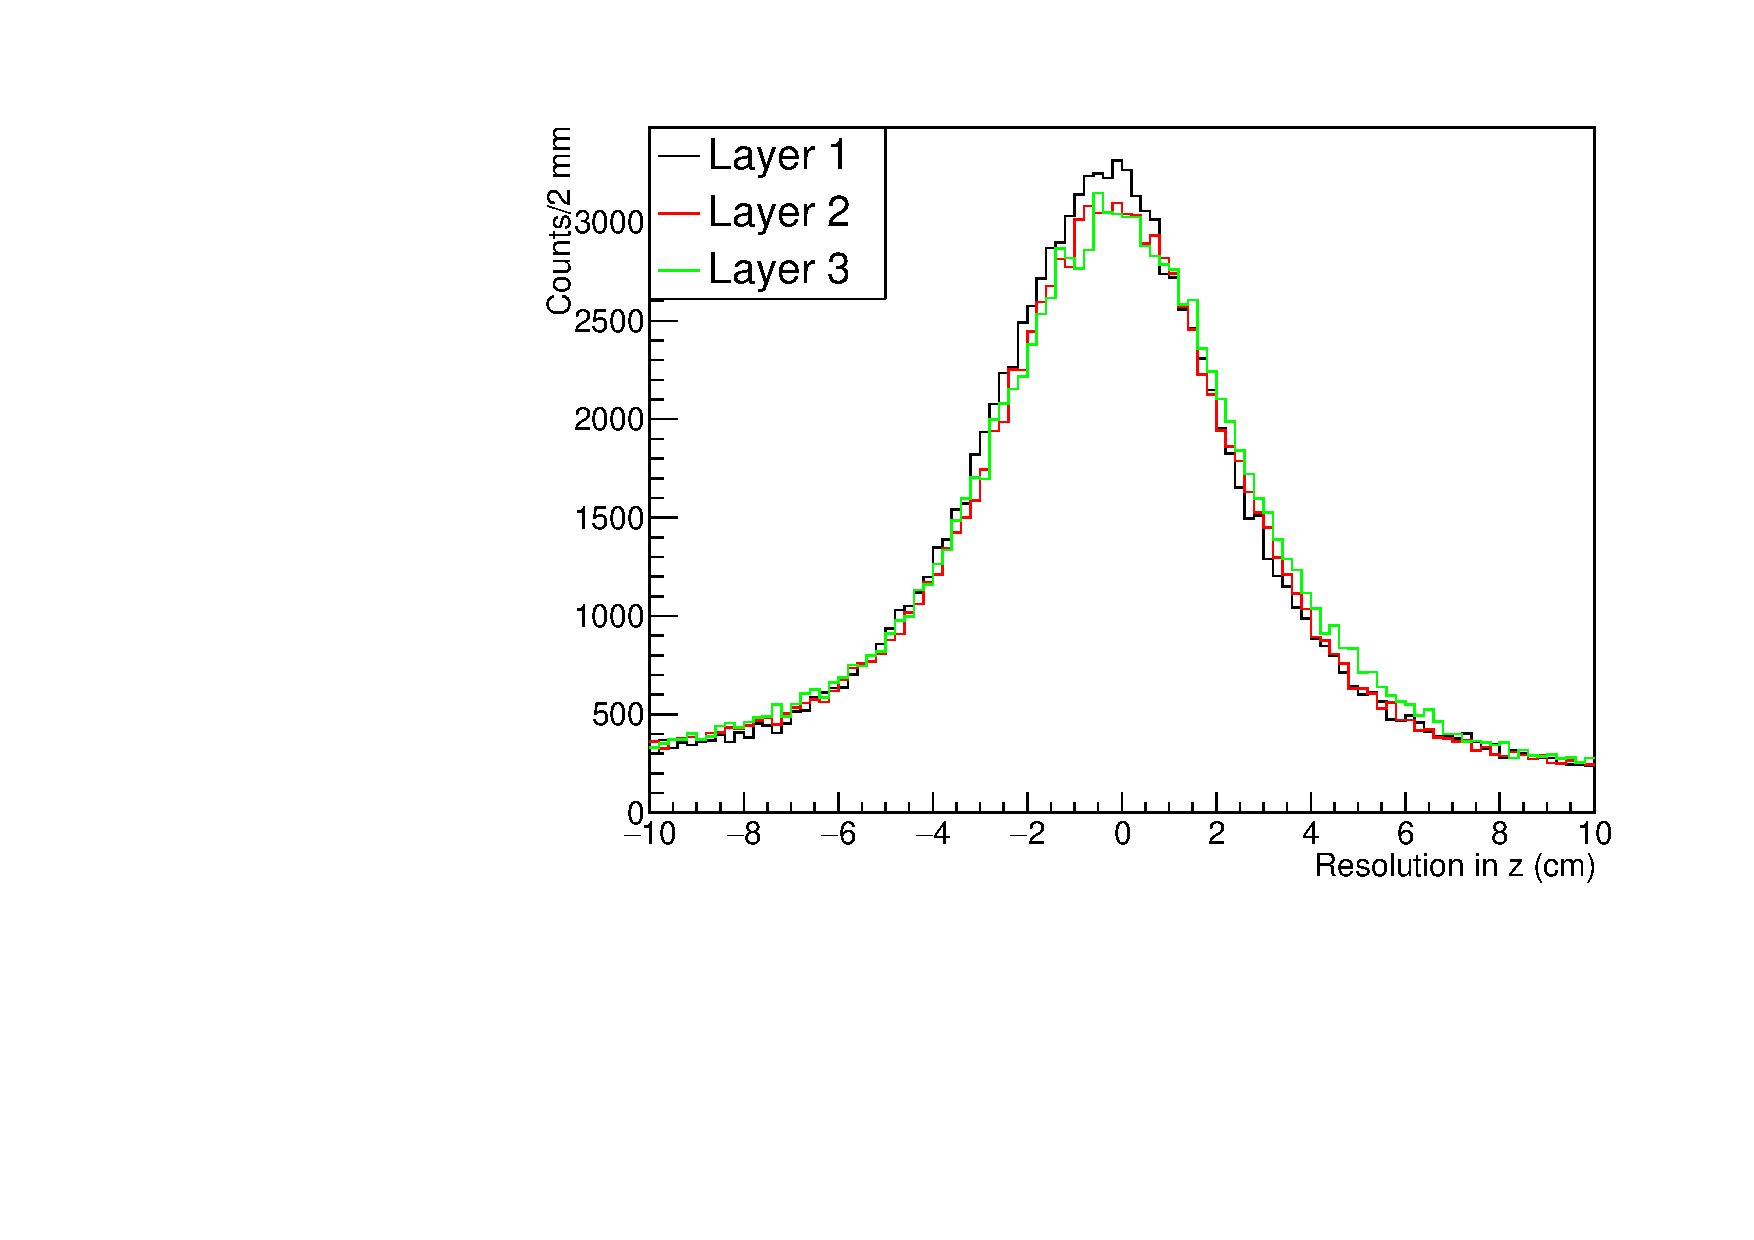
\includegraphics[width=0.45\textwidth]{Figure/canZ.pdf}
\caption {Difference between the $z$ coordinate (along the beamline) computed by the CND and the CVT,for negative tracks in all three CND layers integrated over all paddles.}
\label{fig_performance_deltaz}
\end{center}
\end{figure}

Figure~\ref{fig_performance_edep} shows the energy deposited divided by path length for selected MIPs. It peaks at around the expected value of 2.001~MeV/cm.

\begin{figure}[htb]  
\begin{center}
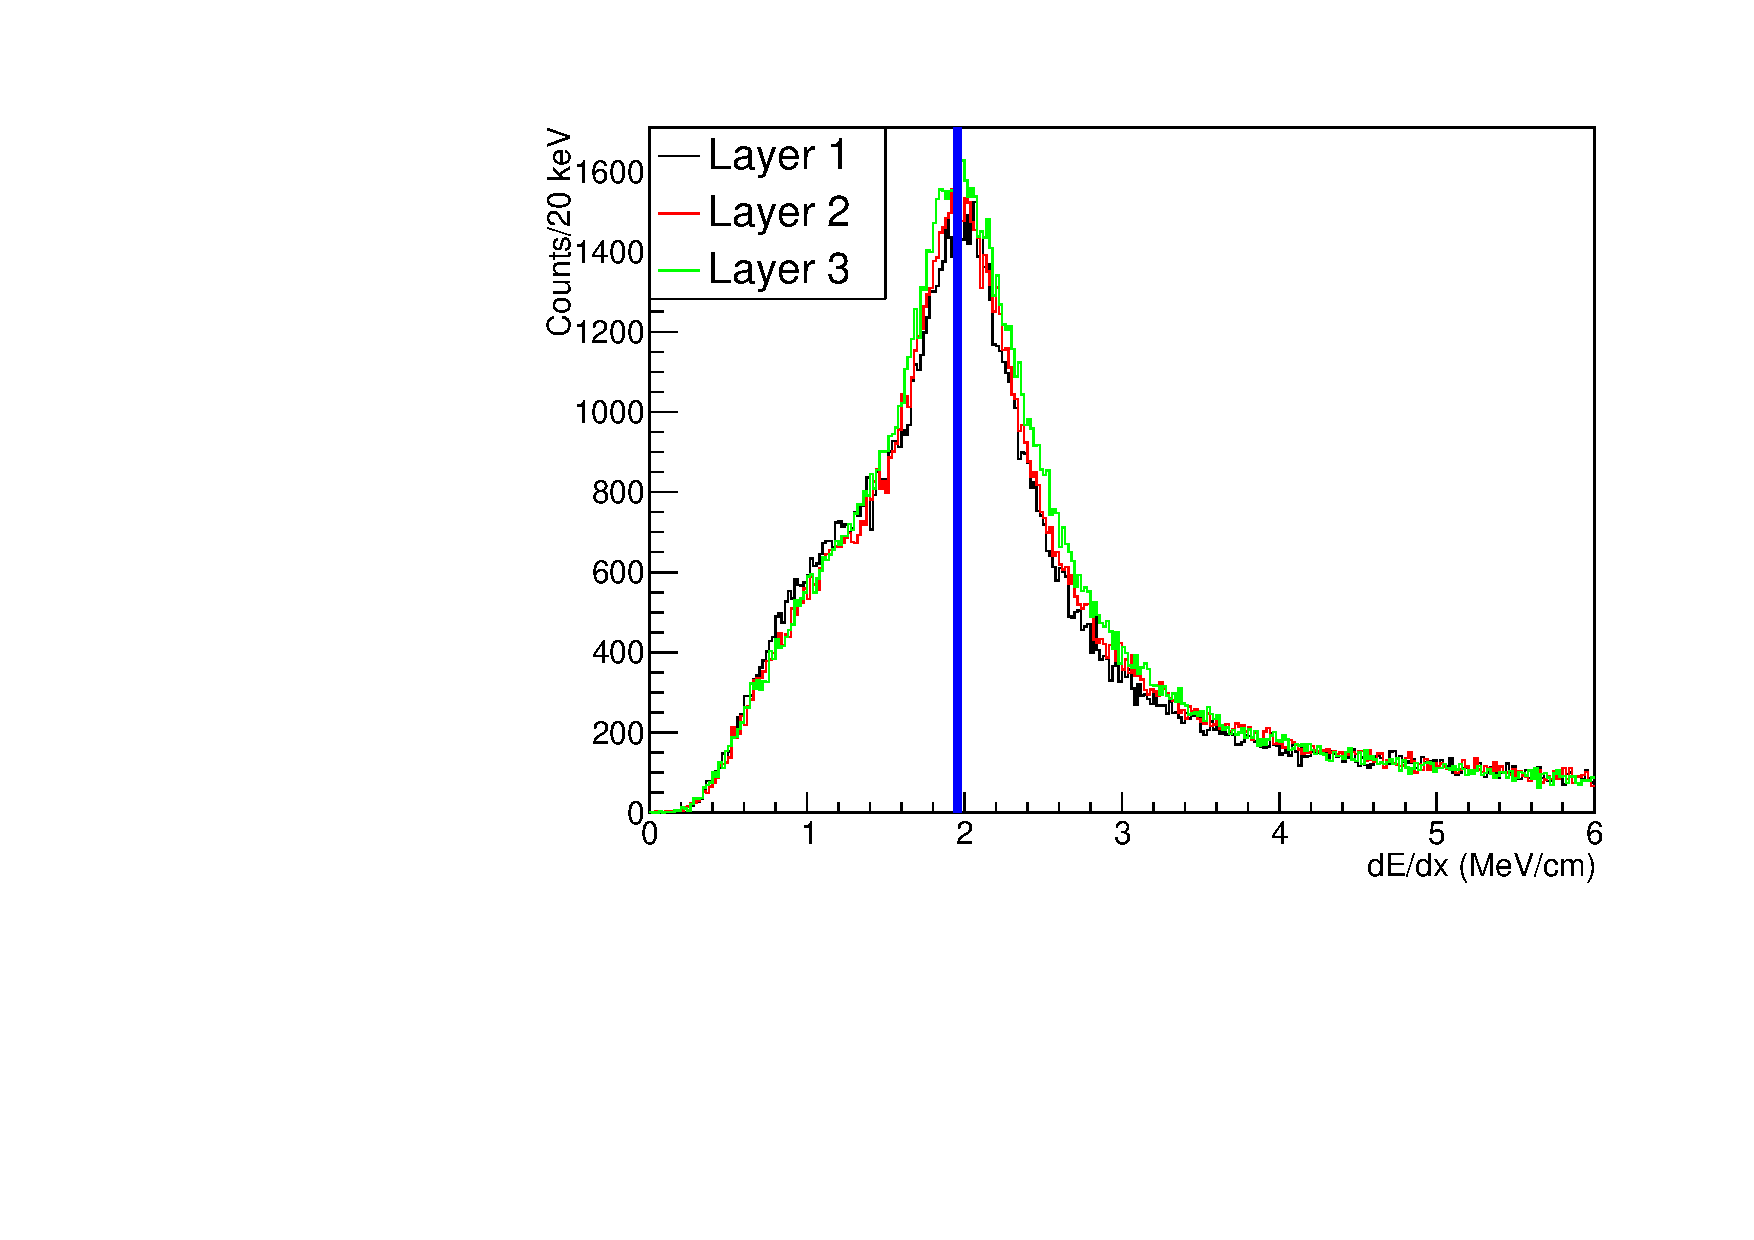
\includegraphics[width=0.45\textwidth]{Figure/canENE.pdf}
\caption {$dE/dx$ for MIPs in the three layers of the CND integrated over all sectors. The blue line indicates the nominal value for the expected energy deposit of a MIP in a centimeter of plastic scintillator.}
\label{fig_performance_edep}
\end{center}
\end{figure}

\subsection{Neutron Detection Efficiency}

The exclusive reaction $e p \to e' n \pi^+$ was analyzed to evaluate the neutron detection efficiency of the CND. The data used were taken with a 7.5-GeV electron beam incident on a liquid-hydrogen target. Events with an electron and a $\pi^+$ in the CLAS12 Forward Detector were selected. The missing mass of the $e' \pi^+ X$ system is plotted versus $\beta_X$ in Fig.~\ref{fig_performance_selection}. The missing particle is required to be in the CLAS12 Central Detector ($\theta>40^\circ$). The effect of this selection is shown in Fig.~\ref{fig_performance_selection}. We apply an additional cut on $\beta$ of the missing neutron ($0.2<\beta_X<0.8$). From this set of $e p \to e' (n) \pi^+$ events, events with a neutron identified by the CND (CND cluster with $E_{dep}>2.5$ MeV, no associated CVT tracks, $\beta<0.8$) were selected. If multiple neutron candidates were detected by the CND, the neutron with the smallest momentum separation from the missing neutron was kept. A cut on $\beta>0.2$ was applied to remove out-of-time hits that could be mistaken as neutrons. Finally, the detected neutron and the missing neutron azimuthal angle difference is constrained to be less than $20^\circ$.

The efficiency was measured in bins of missing neutron polar angle and as a function of missing momentum. For each bin in polar angle and momentum, the efficiency is defined as the ratio of events with a detected neutron to the number of missing neutron events. The result is shown in Fig.~\ref{fig_performance_efficiency}. The detection efficiency extracted from this method is consistent with simulation predictions and with the design specifications of the CND.

\begin{figure}[htb]  
\begin{center}
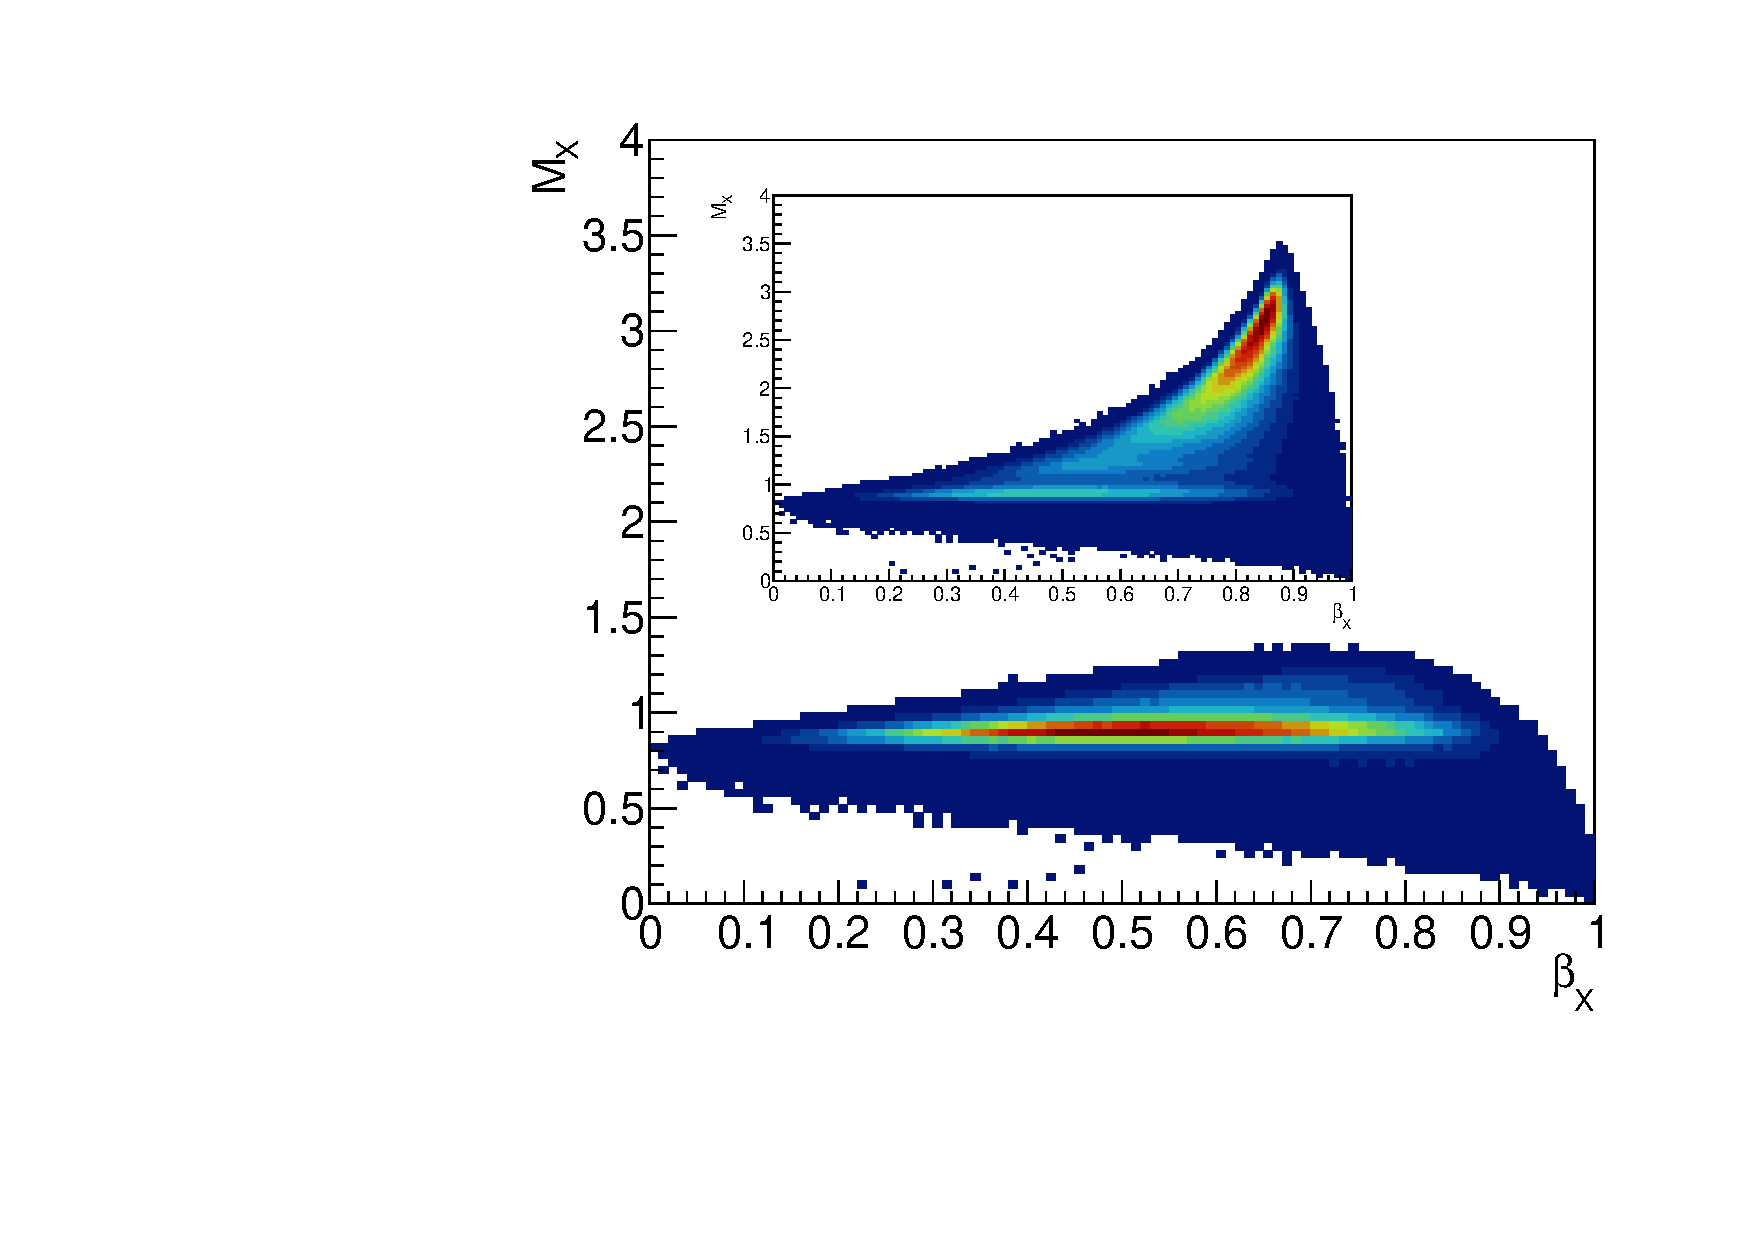
\includegraphics[width=0.5\textwidth]{Figure/SelectionPlots.pdf}
\caption {Missing mass $M_X$ versus $\beta_X$ of the $e p \to e'\pi^+X$ reaction. The outer plot shows the effect of selecting events where the missing particle $X$ is emitted in the CLAS12 Central Detector.}
\label{fig_performance_selection}
\end{center}
\end{figure}

\begin{figure}[htb]  
\begin{center}
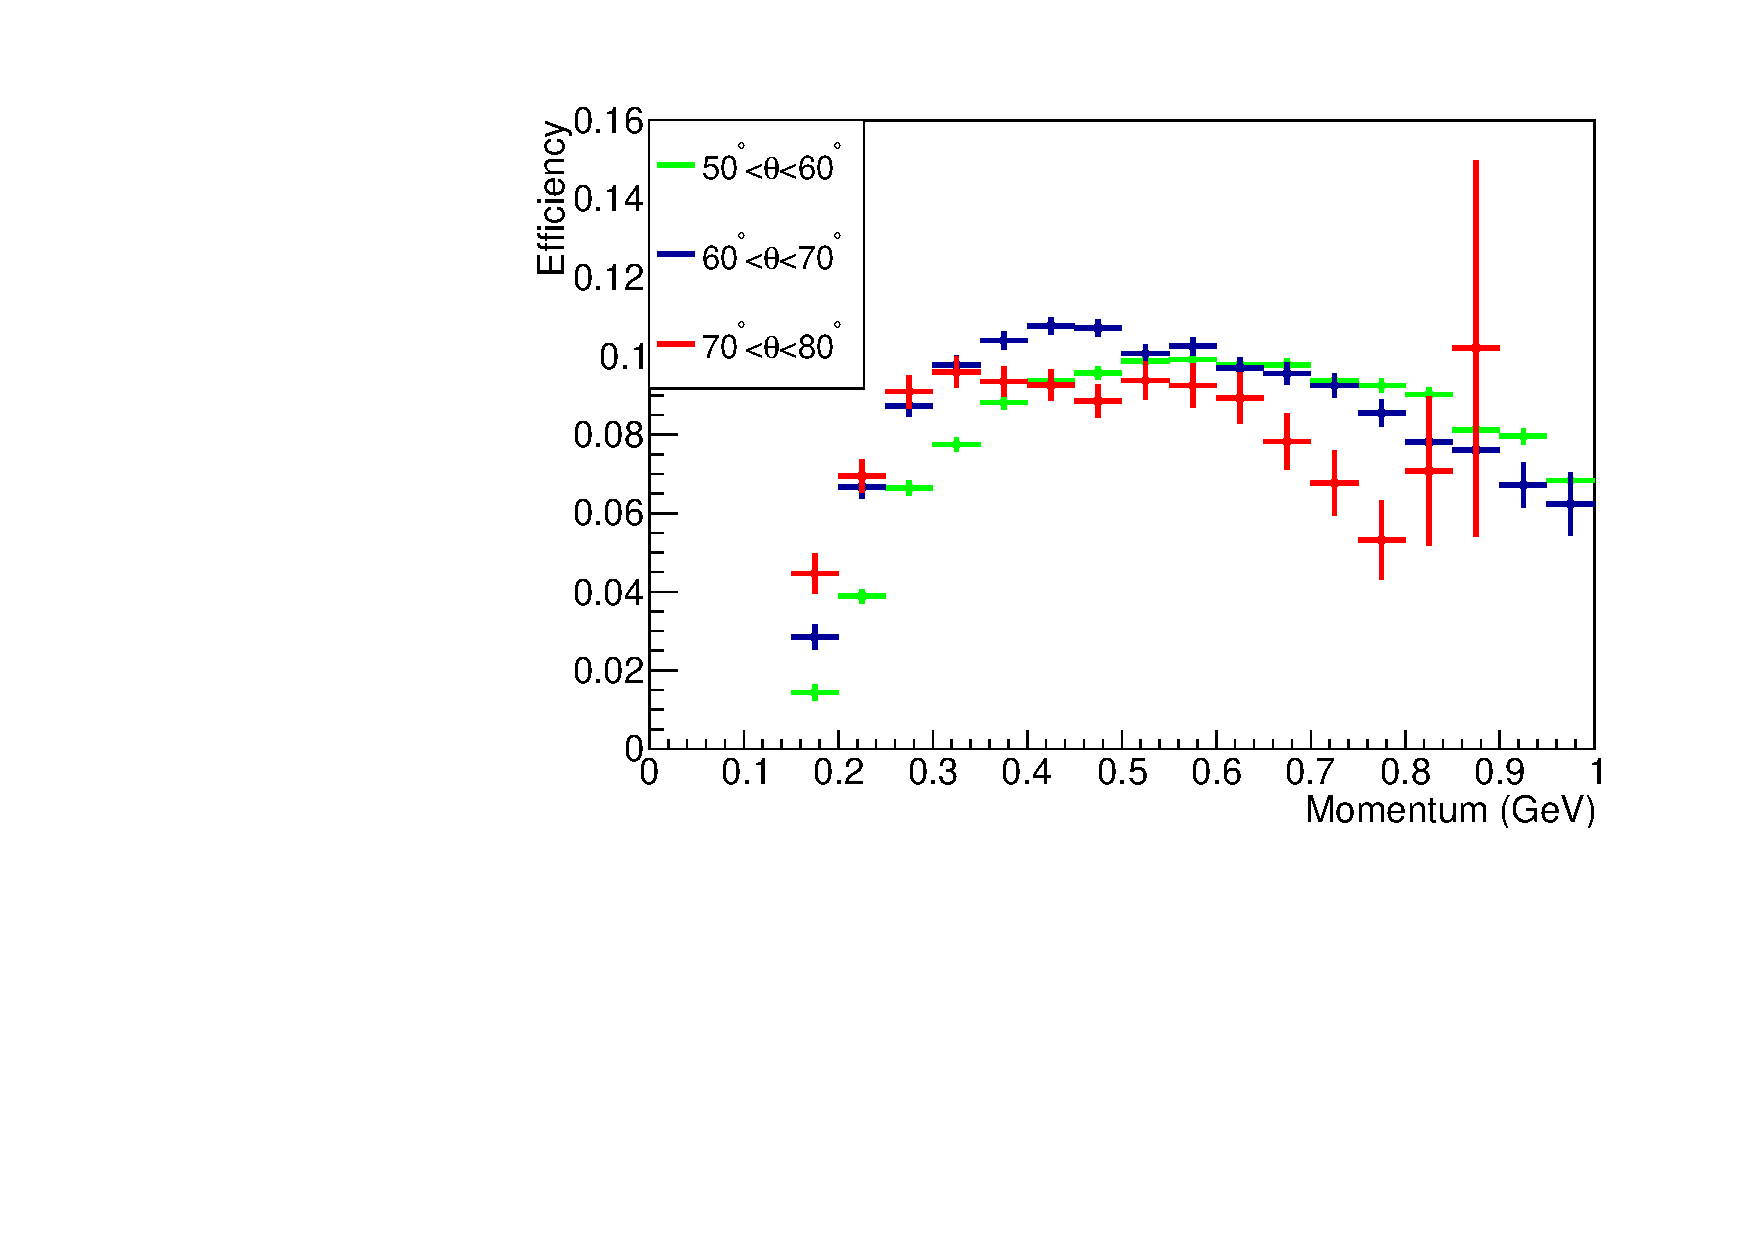
\includegraphics[width=0.5\textwidth]{Figure/newEfficiency.pdf}
\caption {Neutron detection efficiency of the CND as a function of momentum for three bins in polar angle.}
\label{fig_performance_efficiency}
\end{center}
\end{figure}

